\section{Projections}
Given our current project state, we have revised our schedule as follows.
We had to slide back our planned date for finishing the UI/UX and for finalizing
the API. We also compressed our time to polish and debug the site. (Some of this
time was lost due to our schedule delays and some was integrated into the time to
finish scheduling UI/UX).
\begin{figure}[H]
  \centering
  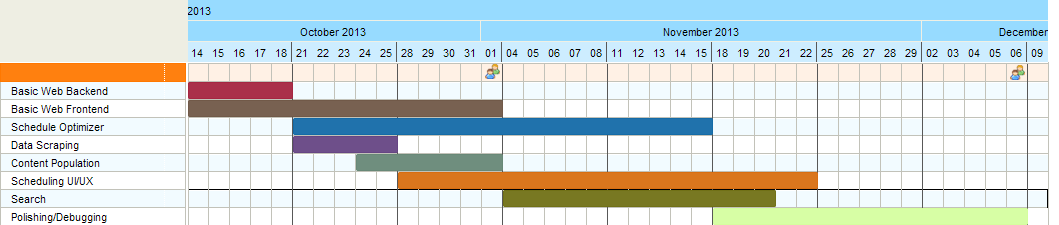
\includegraphics[width=\textwidth]{gantt.png}
  \caption{Original Gantt chart demonstrating proposed project schedule}
%\end{figure}
%\begin{figure}[h!]
%  \centering
  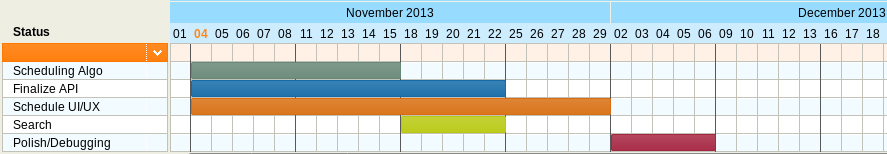
\includegraphics[width=\textwidth]{revised-gantt.png}
  \caption{Revised Gantt chart for next month}
\end{figure}

\section{Recommendations}

We have made significant backend progress, and the remaining work to be done
here consists of finishing the optimization algorithm and
creating the API for the backend code. Thanks to the time initially
allocated to getting the schedule optimizer working, the backend team is
currently slightly ahead of schedule. This is good news, as it will
give them an opportunity to create the best possible scheduling algorithm,
and no significant scheduling changes are required on the backend.

Our frontend has team has somewhat more left to do: although the frontend group
has a barebones UI working, there still exists considerable work required
before the user-facing site and user experience (UX) will be complete, and 
we have added a little extra time for this accordingly.
The frontend team is currently on-schedule to finish as expected initially,
and will hopefully be able to pull ahead of schedule as work on the UI
progresses.

\section{Discussion}

The fact that we're slightly behind overall means that we will have to rush
slightly more than otherwise in order to complete our project. However, our
original Gantt chart left us a decent amount of extra time to account for
eventualities and delays like the ones we reported above, so finishing the
project on time should be entirely feasible.

Because we have assigned the last week purely to polishing and debugging, 
this gives us time to test and make sure everything is perfect before we 
release it to the public. We believe this will also help ensure that our
finished product is high quality and complete.

Overall, the impact of the minor setbacks we've experienced will be minimal,
and we expect to still be able to deliver the same useful, high quality
webapp as promised.
